\section[Fundamental OS]{Fundamental OS}

Understanding how the operating system works is fundamental when developing a
forensics tools. In this thesis, the OS memory management is a required
knowledge. Which is why in this section, we will go through these OS concepts,
pagination, virtual memory, and the OS kernel.

\subsection[Pagination]{Pagination}

Pagination, or paging, is a memory management scheme used by many modern
operating systems. In this scheme, the operating system handles memory by
blocks of constant size. A block of constant size is called a \textit{page}.
The operating system considers a process as a list of pages when using pagination,
and the physical memory RAM (random-access-memory) as a page holder. When
starting a process, the OS will not load the whole process in RAM but only
loads pages that need to be run. When a page in RAM is no longer needed, it
will be removed, \textit{page out}, and replaced by a higher priority page.
The convention \textit{in memory} states that the page is inside RAM, and a
page not inside RAM is said to be \textit{is disk}. In Figure
\ref{fig:pagination} we can see the OS loads some pages of the process in
memory, and the other pages are in disk.

\begin{figure}[h]
  \centering
  \caption{Pagination}
  \label{fig:pagination}
  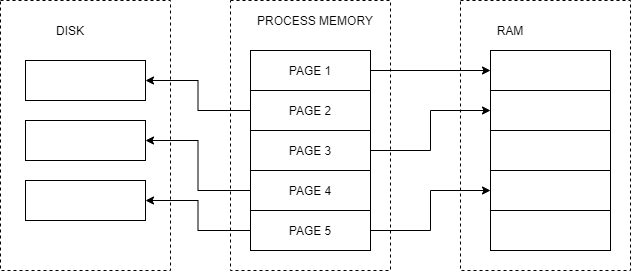
\includegraphics[scale=0.7]{images/pagination.png}
\end{figure}

\subsection[Virtual memory]{Virtual memory}

Virtual memory is a memory management technique where the OS gives an
abstraction level over the addresses indexable by a process. The OS creates a
different address mapping schema for every process running; in other words, two
processes both access the same address results in a different address in RAM.
It is illustrated in Figure \ref{fig:virtualmem}, the two processes have the
same referencing address 0x4000, but in RAM, their addresses are 0x6000 and
0x9000. The address before conversion to RAM address is called virtual address,
and the RAM address is called physical address.

\begin{figure}[h]
  \centering
  \caption{Virtual memory}
  \label{fig:virtualmem}
  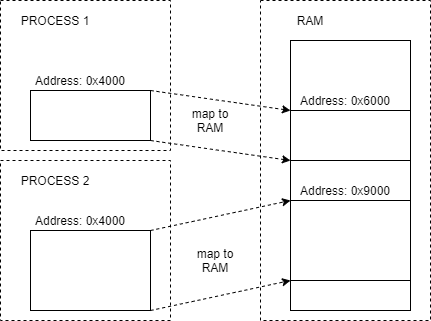
\includegraphics[scale=0.8]{images/virtualmem.png}
\end{figure}

\subsection[Kernel]{Kernel}

The kernel in OS is the program responsible for communicating with the hardware
and controlling other programs. The code for the kernel is loaded in memory
during the machine uptime. The kernel manages critical tasks, including
processes scheduling, memory management, I/O operations.

The kernel handles communication with the hardware through system calls or
\textit{syscall}. There are many implementations to the system call, and the
most common way is by system interrupts.  The kernel will have a syscall table,
which is a table of function pointers. They are called by an interrupt
instruction with the index to the syscall table, as shown in Figure
\ref{fig:syscall}.

\begin{figure}[h]
  \centering
  \caption{System call}
  \label{fig:syscall}
  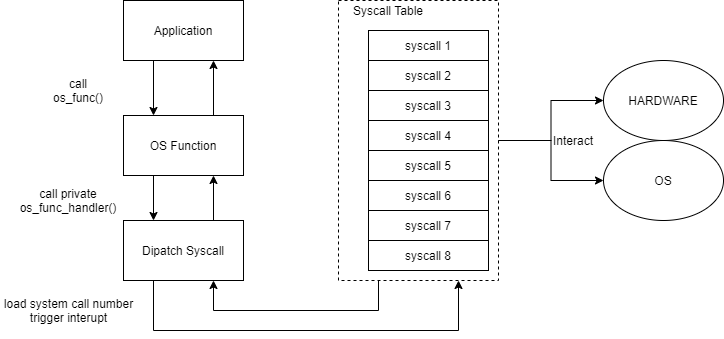
\includegraphics[scale=0.7]{images/syscall.png}
\end{figure}

\subsection[Windows implementation]{Windows implementation}

In Windows 64-bit, pagination is implemented using pages of size 4KB.  Paged
out pages are saved in \texttt{C:\textbackslash\textbackslash Pagefile.sys}.
Virtual memory for every user processes is from 0x0000000000 to 0x7FFFFFFFFFF.
The address from 0x80000000000 to 0xFFFFFFFFFFF is called the system address
space or kernel space.  The system address space is only accessible by the
processes in \textit{kernel-mode}, namely the kernel and kernel drivers.  For
each user process, a separate address space is assigned for the process, but
there is only one system address space and is shared with every kernel
processes running. The user address space and the system address space are
virtual memory, which has to be translated to physical address when access. The
Figure \ref{fig:winimplement} shows the memory layout of the kernel and user
processes memory in Windows 64-bit systems. While the user process can not
access system address space, kernel processes can access any virtual page.

\begin{figure}[h]
  \centering
  \caption{Windows memory layout}
  \label{fig:winimplement}
  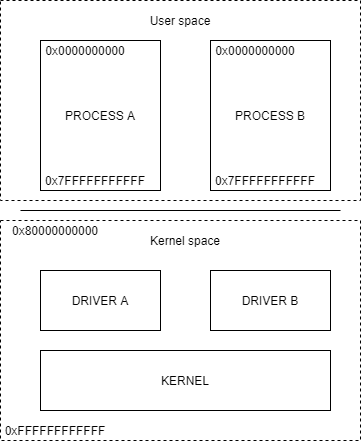
\includegraphics[scale=0.7]{images/winimplement.png}
\end{figure}

Syscall in Windows is called in two ways, and both implemented with a system
call table. The first way is done by interrupting the code 0x2e, and the second
way is using the instruction sysenter/syscall. Both ways receive the index to
the system call table in register edx.
